





\section{Examples}

%%%%%%%%%%%%%%%%%%%%%%%%%%%%%%%%%%%%%%%%%%%%%%%%%%%%%%%%%%%%%%%%%%%%%%%%%%%%%%%%

Figure \ref{fig_add} illustrates an algebraic decision diagram (ADD).

\begin{figure}%[H]
  \centering
  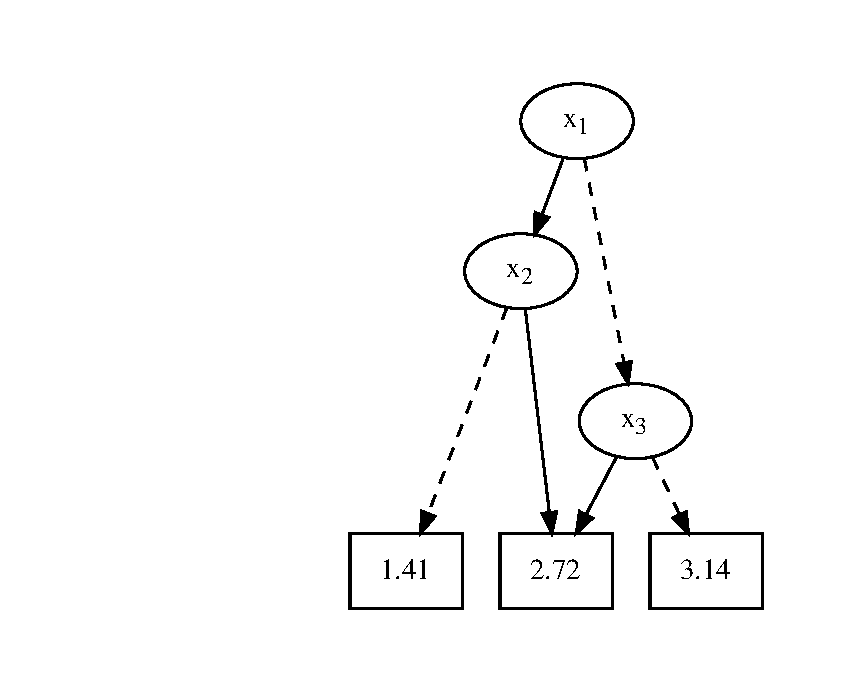
\includegraphics[
    % height=2in,
    trim={2in .5in .1in .5in} % <left> <lower> <right> <upper>
  ]
  {figures/4/ADD.pdf}
  \caption{
    The directed graph $G$ of an ADD with variable set $X = \set{x_1, x_2, x_3}$, carrier set $S = \R$, and diagram variable order $\pi(x_i) = i$ for $i = 1, 2, 3$.
    If an edge from an oval node is solid (respectively dashed), then the corresponding Boolean variable is assigned 1 (respectively 0).
  }
\label{fig_add}
\end{figure}
